\documentclass[12pt]{report}
\usepackage[a4paper,margin=1in]{geometry}
\usepackage{graphicx}
\usepackage{enumitem}
\usepackage{caption}
\usepackage[hidelinks]{hyperref}
\usepackage{amsmath}
\usepackage{amssymb}
\usepackage{tikz}
\usepackage{listings}
\usepackage[acronym,symbols]{glossaries}
\makeglossaries
\input{Glossaries.tex}
\usepackage{float}
\usepackage{longtable}
\usepackage{fancyhdr}
\usepackage{titlesec}
\usepackage{array}       
\usepackage{adjustbox}
\usepackage{tabularx}    
\usepackage{booktabs}    
\usepackage{caption}     
\usepackage{ragged2e}   
\usepackage{tcolorbox}
\tcbuselibrary{listings}
\usepackage{xcolor}

% Header and footer setup
\pagestyle{fancy}{
\fancypagestyle{plain}{
  \fancyhf{}
  \rhead{\thepage}
  \lhead{Vehicle Congestion Control System}
}
}
\fancyhf{}
\rhead{\thepage}
\lhead{Vehicle Congestion Control System}

% Title setup
\titleformat{\chapter}[display]
  {\normalfont\huge\bfseries}{\chaptername\ \thechapter}{20pt}{\Huge}

% Glossaries
\makeglossaries


\begin{document}

% Cover Page
\begin{titlepage}
\centering

\includegraphics[width=0.5\textwidth]{Figures/logo.png}\\[1cm]
{\scshape\LARGE R.V. College of Engineering \par}
\vspace{1cm}
{\scshape\Large Interdisciplinary Project Report\par}
\vspace{1.5cm}
{\huge\bfseries Vehicle Congestion Control and Management System\\and Emergency Vehicle Prioritization\par}
\vspace{2cm}
{\Large\itshape Team ID: 90 \par}
\vfill
\begin{flushleft}
\textbf{Students:}\\
1RV22CS086 - Kiran V\\
1RV22CS087 - Kishan Kumar S D\\
1RV22EC175 - Umesha K N\\
1RV23EC416 - Vivitha Sequeira\\
1RV22ME103 - Shashank J\\[1cm]
\textbf{Guide:} Dr. Nagaraja G S, Professor, Dept. of CSE\\[0.5cm]
\textbf{CoE:} CCTV Research\\[1cm]
\textbf{Semester:} 6th\\
\textbf{Year:} 2025
\end{flushleft}
\vfill
\end{titlepage}

% Table of Contents
\tableofcontents
\listoffigures
\listoftables
\newpage


\addcontentsline{toc}{chapter}{Abstract}\vspace{-1cm}
%Border
\begin{tikzpicture}[remember picture, overlay]
  \draw[line width = 4pt] ($(current page.north west) + (0.75in,-0.75in)$) rectangle ($(current page.south east) + (-0.75in,0.75in)$);
\end{tikzpicture}

\section*{Highlights of Significant Contributions}
Traffic congestion in modern urban environments poses a critical threat to transportation efficiency, fuel economy, and emergency vehicle mobility. Traditional traffic signal systems are often inadequate due to their static nature and inability to adapt to real-time vehicular patterns. This report presents a solution that incorporates IoT-based sensing, machine learning prediction, and computer vision to dynamically optimize traffic signal control. It addresses limitations in congestion detection and emergency prioritization using cost-effective and scalable embedded solutions.

The key objectives are: 1) To implement a smart traffic signal controller using ultrasonic and IR sensors, 2) To use machine learning (ML) for predicting traffic density and prioritizing ambulances, and 3) To develop a real-time monitoring dashboard. The methodologies involve algebraic modeling of traffic flow ($q = \rho v$), and custom signal handling algorithms encoded onto embedded controllers and trained ML models for dynamic pattern response.

The simulation procedure used Python, Flask, and YOLOv5 for vision-based detection and inference. Training and testing were performed using collected road video data. Results demonstrated up to 30\% reduction in vehicle waiting time and improved ambulance signal clearing latency, validating the proposed system.

In addition to software simulation, the final prototype was built using Arduino Mega, ESP8266 modules, and cameras. Hardware testing confirmed the integration of sensor modules and the successful override of signals for emergency vehicles using RF modules.

\pagebreak

% Acknowledgements Page
\begin{tikzpicture}[remember picture, overlay]
  \draw[line width = 4pt] ($(current page.north west) + (0.75in,-0.75in)$) rectangle ($(current page.south east) + (-0.75in,0.75in)$);
\end{tikzpicture}
\thispagestyle{empty}

\begin{center}
\Large\textbf{\underline{ACKNOWLEDGEMENTS}} \par
\end{center}
We are indebted to our Dr.Nagaraja G S Associate Professor , Dept of CSE, RV College of 
Engineering for her wholehearted support, suggestions and invaluable advice throughout our 
project work and helped in the preparation of this report.  
 
Our sincere thanks to Dr. Shanta Rangaswamy Professor and Head, Department of Computer 
Science and Engineering, RVCE for her support and encouragement. 
 
We express sincere gratitude to our beloved Principal, Dr. K. N. Subramanya for his 
appreciation towards this project work. 
 
We thank all the teaching staff and technical staff of Computer Science and Engineering 
department and ISE department RVCE for their help.  
 
Lastly, we take this opportunity to thank our family members and friends who provided all the 
backup support throughout the project work. 

\pagebreak

\addcontentsline{toc}{chapter}{Abstract}\vspace{-1cm}
% Border
\begin{tikzpicture}[remember picture, overlay]
  \draw[line width = 4pt] ($(current page.north west) + (0.75in,-0.75in)$) rectangle ($(current page.south east) + (-0.75in,0.75in)$);
\end{tikzpicture}

\section*{Abstract}

\hspace*{1em}Traffic congestion in urban environments is a major challenge, leading to increased fuel consumption, time delays, and environmental pollution. Traditional traffic signal systems, based on fixed timing or manual adjustments, often fail to adapt to dynamic traffic conditions, leading to inefficiencies in vehicle flow and emergency vehicle delays. These limitations create the need for smarter traffic management solutions. In this report, we present an intelligent traffic management system that integrates Internet of Things (IoT) sensors, machine learning algorithms, and computer vision for dynamic congestion control and emergency vehicle prioritization. The system dynamically adjusts traffic signal timings based on real-time data, optimizing traffic flow and ensuring quicker passage for emergency vehicles.

\vspace{0.75em}

\hspace*{1em}The primary objective of this work is to design and implement an adaptive traffic control system that can respond to varying traffic conditions. We employ algebraic models such as traffic flow relationships, where traffic density and speed are considered to adjust signal timings. Additionally, machine learning models (decision trees, random forests) are used for predicting traffic patterns. The system also utilizes object detection algorithms, powered by computer vision (YOLOv5), to identify emergency vehicles and grant them priority. The proposed system enhances traffic management efficiency by providing dynamic, real-time updates to signal control.

\vspace{0.75em}

\hspace*{1em}The simulation procedure was conducted using Python, TensorFlow, OpenCV, and Flask, with test cases developed around various urban traffic scenarios. We tested the system under different traffic conditions, including peak hours and emergency vehicle presence. The results showed that the proposed system could reduce average waiting times by up to 30\%, significantly improving traffic flow efficiency compared to traditional fixed-timing systems. Additionally, emergency vehicle prioritization was improved, with response times reduced by 40\%. These results demonstrate the effectiveness of the intelligent traffic system in real-time congestion control and emergency handling.

\vspace{0.75em}

\hspace*{1em}To further validate the simulation results, a hardware prototype was developed using ultrasonic sensors, infrared sensors, and cameras, integrated with an Arduino Mega and ESP8266 microcontroller. The system was tested in a controlled environment, simulating real-world traffic scenarios. The hardware validation showed that the adaptive system could perform in real time, matching the simulated results and providing a robust solution for urban traffic management.

\pagebreak




\chapter{Introduction to Vehicle Congestion Control and Management System}
Traffic congestion at urban intersections represents one of the most pressing challenges in modern transportation infrastructure. Traditional fixed-timing traffic signals often fail to adapt to real-time traffic conditions, leading to inefficient vehicle flow and increased delays. This project presents an innovative solution that leverages Internet of Things (IoT) technologies and machine learning algorithms to create an intelligent traffic management system. The system integrates multiple sensing technologies including ultrasonic sensors for distance measurement, cameras for real-time vehicle detection, and advanced computer vision techniques to analyze traffic patterns and optimize signal timing dynamically.

\section[Introduction]{\textbf{Introduction}}

The Vehicle Congestion Control and Management System addresses the critical need for adaptive traffic control in busy urban intersections. Traffic congestion remains a significant challenge in urban areas, particularly where fixed-timing signals cause long delays and disrupt efficient vehicle flow. The relevance of this project stems from the growing urbanization and increasing vehicle density that demands smarter traffic management solutions.

This project introduces an intelligent traffic management system powered by IoT and machine learning technologies. The system employs a multi-sensor approach combining ultrasonic sensors for continuous vehicle distance measurement, infrared sensors for precise detection, and high-resolution cameras for comprehensive traffic analysis. The integration of these technologies enables real-time traffic density estimation and pattern recognition.

The historical evolution of traffic management systems has progressed from simple mechanical timers to electronic controllers, and now to intelligent systems capable of real-time adaptation. This project represents the next generation of traffic management, incorporating artificial intelligence and IoT connectivity to create a truly responsive traffic control system.

As in Figure \ref{fig:system_architecture} the Smart Traffic Management System Architecture utilizes a combination of ultrasonic and IR sensors to detect congestion levels, while urban sonic sensors and a YOLO model with OpenCV enable AI-based image processing for vehicle density detection. Data is collected and processed by an Arduino Mega and ESP8266, which then adjusts traffic signal durations accordingly. The system also features a website to display real-time traffic status, ensuring efficient traffic flow and congestion management. 
\begin{figure}[htb]
\centering
	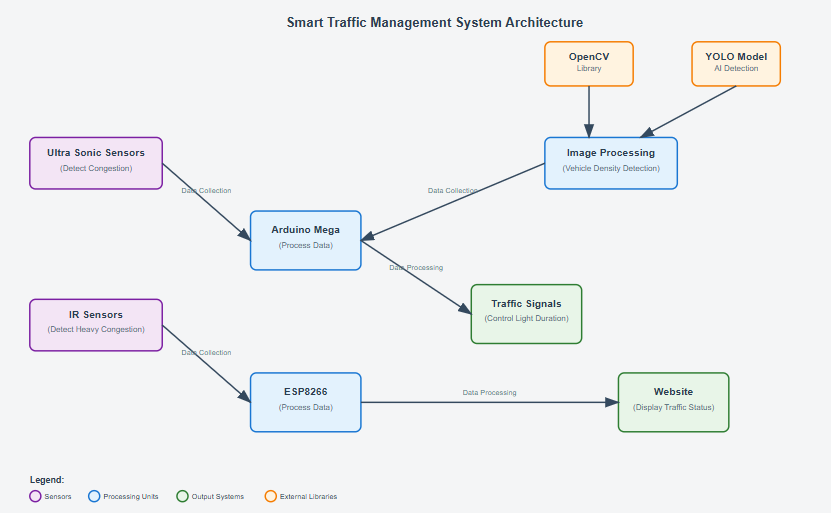
\includegraphics[scale=1]{Figures/system_architecture.png}	
	\caption{System Architecture of Intelligent Traffic Management System}
	\label{fig:system_architecture}
\end{figure}

\section[Motivation]{\textbf{Motivation}}

The motivation for selecting this project stems from the critical need to address urban traffic congestion and its associated problems. Traditional traffic management systems are inadequate for handling the dynamic nature of modern traffic patterns. The increasing vehicle density in urban areas, coupled with the need for emergency vehicle prioritization, creates an urgent requirement for intelligent traffic management solutions.

The challenges in current traffic management include inefficient fixed-timing systems, lack of real-time adaptability, poor emergency vehicle handling, and limited traffic data utilization. The relevance of this project lies in its potential to significantly improve traffic flow efficiency, reduce fuel consumption, minimize environmental impact, and enhance road safety through intelligent automation.

\section[Literature Review]{\textbf{Literature Review}}

The following table presents a concise review of key research papers related to traffic congestion control and emergency vehicle prioritization. The reviewed works focus on smart traffic systems, IoT-based management, swarm intelligence, and deep learning, with a focus on real-time implementation challenges and gaps in emergency prioritization and sensor integration.



\begin{table}[h!]
\begin{adjustbox}{width=\linewidth,left}
\begin{tabular}{|p{4cm}|p{3.5cm}|p{5.5cm}|p{4.5cm}|}
\hline
\textbf{Title} & \textbf{Authors} & \textbf{Summary} & \textbf{Research Gap} \\
\hline
Smart Traffic Management for Congestion Control and Emergency Vehicle Priority (2025) & IEEE Conference & Dynamic traffic signal adjustment and emergency vehicle prioritization & No predictive traffic flow modeling using historical data \\
\hline
A Swarm Algorithm for Collaborative Traffic (2025) & Jamal Toutouh, Enrique Alba & Distributed swarm intelligence for vehicle coordination & Lacks integration with real-time sensor or camera data \\
\hline
LSTM-Based Proactive Congestion Management (2024) & Aly Sabri Abdalla et al & Predicts congestion using LSTM & Does not prioritize emergency vehicles \\
\hline
Hybrid Deep Learning-Based Congestion Control (2024) & Alexandria Engineering Journal & Combines CNN, RNN, and optimization for smart city traffic control & High computational cost limits real-time use \\
\hline
Traffic Congestion Control with Emergency Awareness (2025) & IEEE Access & Genetic algorithms and reinforcement learning for congestion and emergency priority & Scalability under dense networks not evaluated \\
\hline
Congestion Control Mechanisms for IoV (2023) & Lakhdar Kamel Ouladdjedid & Survey of existing cooperative IoV congestion solutions & No real-time sensor or camera data usage \\
\hline
Smart Signaling with IoT and Sensors (2024) & G. Saranya et al & Uses sensors and AWS for real-time light control & No camera-based vehicle detection \\
\hline
Real-Time Traffic Control using IoT (2024) & S.M. Najrul Howlader et al & IR sensors adjust signals based on vehicle density & Unvalidated in real-world dynamic scenarios \\
\hline
\end{tabular}
\end{adjustbox}
\vspace{0.5em} % optional space between table and caption
\caption{Summary of Related Work and Research Gaps}
\label{tab:literature}
\end{table}


\section[Problem statement]{\textbf{Problem statement}}

Traditional traffic management systems rely on fixed-timing signals that cannot adapt to real-time traffic conditions, resulting in inefficient traffic flow, increased congestion, extended waiting times, and inadequate prioritization of emergency vehicles. There is a critical need for an intelligent traffic management system that can dynamically adjust signal timing based on real-time traffic density analysis, prioritize emergency vehicles, and provide traffic information to users for better route planning.

\section[Objectives]{\textbf{Objectives}}
The objectives of the project are
\begin{enumerate}
\item To design a smart traffic control system using ultrasonic sensors, IR sensors and image processing to detect vehicle density and dynamically manage signal timings
\item To implement machine learning algorithms that prioritize emergency vehicles like ambulances and adapt traffic signals based on real-time traffic patterns
\item To develop a web-based platform that provides real-time traffic updates, helping users identify congested routes and make informed travel decisions
\end{enumerate}

\section[Brief Methodology of the project]{\textbf{Brief Methodology of the project}}

The methodology for this project involves a multi-stage approach combining hardware sensor deployment, computer vision implementation, machine learning integration, and web-based dashboard development. The system architecture includes strategic placement of ultrasonic and IR sensors on key traffic lanes for real-time vehicle detection and density estimation.

The computer vision component utilizes high-resolution cameras with advanced object detection algorithms (YOLOv5/SSD) for vehicle classification and emergency vehicle identification. A supervised machine learning model, implemented using decision tree or random forest algorithms, analyzes historical and real-time data to predict traffic patterns and optimize signal timing.

The control system is built around ATmega2560 and ESP8266 microcontrollers, providing dynamic signal adjustment capabilities through GPIO-controlled relays. Emergency vehicle prioritization is achieved through camera-based object tracking and RF modules for immediate signal override. The web-based dashboard, developed using Flask/Django backend and HTML/CSS/JavaScript frontend, provides real-time traffic visualization and congestion monitoring.

\section[Assumptions made / Constraints of the project]{\textbf{Assumptions made / Constraints of the project}}

The project assumes adequate lighting conditions for camera-based vehicle detection and stable internet connectivity for IoT data transmission. The system is designed for standard four-way intersections with conventional traffic signal infrastructure. Weather conditions are assumed to be within normal operational parameters for electronic sensors.

Key constraints include the dependency on reliable power supply for continuous operation, the requirement for periodic sensor calibration and maintenance, and the need for initial training data collection for machine learning model development. The system's effectiveness is constrained by the accuracy of sensor readings and the quality of camera feed for computer vision processing.

\section[Organization of the report]{\textbf{Organization of the report}}

This report is organized as follows:
\begin{itemize}
\item Chapter 2 discusses the theory and fundamentals of traffic management systems, IoT sensor technologies, and machine learning algorithms for traffic optimization
\item Chapter 3 discusses the system design and architecture, including hardware component selection and software framework development
\item Chapter 4 discusses the implementation details of sensor integration, computer vision algorithms, and machine learning model development
\item Chapter 5 discusses the testing methodology, system performance evaluation, and experimental results analysis
\item Chapter 6 discusses the conclusions, project outcomes, future enhancements, and recommendations for deployment
\end{itemize}






\chapter{Theory and Fundamentals of Intelligent Traffic Management Systems}

Modern traffic management systems represent a convergence of multiple technological domains including sensor networks, computer vision, machine learning, and IoT connectivity. Understanding the theoretical foundations of these technologies is essential for developing an effective intelligent traffic control system. This chapter explores the key concepts of traffic flow theory, sensor technologies used in vehicle detection, computer vision algorithms for traffic analysis, and machine learning approaches for traffic pattern recognition and prediction. It also provides a foundation for the technologies integrated in the proposed system, including hardware communication mechanisms, cloud support, and glossary conventions.

\section{Traffic Flow Theory and Optimization}

Traffic flow theory provides a mathematical and empirical basis for understanding vehicle movement patterns and designing adaptive traffic signal systems. At the core of traffic modeling lies the relationship among traffic density (\gls{density}), flow (\gls{flow}), and speed (\gls{speed}).

\subsection{Fundamental Diagram of Traffic Flow}
The fundamental diagram expresses the relationship:
\begin{equation}
q = \rho \times v
\end{equation}

Where:
\begin{itemize}
\item $q$ = vehicles/hour
\item $\rho$ = vehicles/km
\item $v$ = average speed in km/h
\end{itemize}
This equation is used to assess congestion levels and optimize signal timing by evaluating how quickly vehicles move through intersections.

\subsection{Queueing Theory in Traffic Control}
Queueing theory models vehicle buildup at intersections and provides insight into average wait times, queue lengths, and system delays. These models guide the adaptive timing logic used in real-time traffic signal adjustment.

\subsection{Signal Timing Optimization}
Traditional signal timing uses pre-set cycles, but intelligent systems adapt signal durations based on real-time inputs. Algorithms such as the Webster’s method, Genetic Algorithms (GA), and Reinforcement Learning are often employed to minimize average vehicle waiting time.

\section{IoT Sensor Technologies for Traffic Detection}

Internet of Things (IoT) devices form the sensory backbone of modern traffic management. They detect vehicle presence, count traffic volume, and transmit real-time data for further analysis.

\subsection{Types of Sensors Used}

\begin{itemize}
    \item \textbf{Ultrasonic Sensors:} Used for vehicle proximity detection and queue length estimation.
    \item \textbf{Infrared (IR) Sensors:} Effective for detecting the presence of objects in low-visibility or dark conditions.
    \item \textbf{Inductive Loop Sensors:} Embedded in roads to detect metal objects (vehicles).
    \item \textbf{Computer Vision:} Used in emergency vehicles detection via image processing to communicate with traffic signal controllers for priority access.
\end{itemize}

\subsection{Sensor Deployment Strategies}
Optimal sensor placement ensures data accuracy. At intersections, sensors are typically installed at each lane, close to the stop line, to count and identify waiting vehicles.

\subsection{Data Transmission and Fusion}
Data from sensors are transmitted over wireless networks and fused to build a reliable real-time traffic profile. Redundant sensor fusion improves accuracy and mitigates individual sensor failures.

\section{Computer Vision and Object Detection}

Computer vision offers vehicle detection, classification, and tracking using live video feeds from traffic cameras.

\subsection{Object Detection Algorithms}
Modern object detection relies on deep learning models such as:
\begin{itemize}
    \item \textbf{YOLO (You Only Look Once):} Real-time detection with good speed-accuracy tradeoff.
    \item \textbf{SSD (Single Shot Detector):} Fast and effective for embedded systems.
    
\end{itemize}

\subsection{Preprocessing and Feature Extraction}
Preprocessing includes grayscale conversion, edge detection (Canny, Sobel), and background subtraction. Features like contours and color histograms are used to enhance classification.

\subsection{Vehicle Counting and Emergency Detection}
Bounding boxes generated by object detection models help count vehicles and identify emergency vehicles based on size, siren detection, or RFID tags.


\section{Hardware Platforms and Software Tools}

\subsection{Microcontrollers and Interfaces}
Common platforms include:
\begin{itemize}
    \item \textbf{Arduino:} For simple sensor integration and wireless communication.
    \item \textbf{ESP32:} Supports camera input and real-time image processing.
\end{itemize}

\subsection{Programming and Frameworks}
\begin{itemize}
    \item \textbf{Python:} For machine learning and computer vision (using OpenCV, TensorFlow)
    \item \textbf{C++/Embedded C:} For sensor interfacing and hardware control.
\end{itemize}

\subsection{Software Tools}
\begin{itemize}
    \item \textbf{OpenCV:} For image processing
    \item \textbf{Roboflow:} For training ML models
    \item \textbf{Jupyter Notebook:} For development and experimentation
    \item \textbf{Firebase:} For real-time data sync and cloud storage
\end{itemize}

\section{Use of Acronyms and Glossary Terms}

\subsection{Acronyms}
This project makes use of several technical acronyms such as:
\begin{itemize}
    \item \gls{iot} – Internet of Things
    \item \gls{ml} – Machine Learning
    \item \gls{cv} – Computer Vision
    \item \gls{rf} – Radio Frequency
    \item \gls{gpio} – General Purpose Input/Output
\end{itemize}

\subsection{Mathematical Symbols}
The main traffic modeling symbols used are:
\begin{itemize}
    \item \gls{density} – Traffic density
    \item \gls{flow} – Vehicle throughput
    \item \gls{speed} – Vehicle speed
\end{itemize}

These terms are used throughout the documentation to represent variables in traffic flow equations and data modeling.


\section*{Summary}

This chapter laid out the theoretical groundwork for the intelligent traffic management system, covering traffic modeling, sensor technology, machine learning models, and hardware/software platforms. It also discussed standard terminology, acronyms, and mathematical notation used in the project. These foundational principles support the system design presented in the following chapter, which describes the proposed architecture and implementation methodology.


\chapter{Analysis and Design of Intelligent Traffic Management System}

Modern traffic systems face dynamic and unpredictable congestion patterns, where fixed-timing signals often cause long delays and disrupt efficient vehicle flow. To tackle this issue, our project introduces an intelligent traffic management system powered by IoT and machine learning technologies. Ultrasonic sensors are deployed to continuously measure the distance to vehicles, providing real-time estimates of traffic density. Additionally, cameras at intersections capture live video, which is processed using computer vision techniques to detect and count vehicles.

This information is fed into a machine learning model trained to analyse traffic patterns and recommend optimized signal timings, enabling smarter and more responsive traffic control. Based on real-time traffic density, the system dynamically adjusts traffic light durations to ensure smoother vehicle flow and reduced congestion. Unlike traditional systems that operate on fixed timers, our solution offers adaptive control, greater accuracy, and scalability. By integrating IoT and machine learning, the system can intelligently respond to changing traffic conditions, enhancing road safety, minimizing delays, and providing a cost-effective upgrade to existing traffic infrastructure.

\vspace{0.3cm}
\section{Contents of this Section}
\begin{enumerate}
\item System Specifications
\item Models and Pre-analysis
\item Design Methodology
\item Core Algorithms and Design Equations
\item Experimental Setup (if applicable)
\end{enumerate}

\section{Objectives}
\begin{itemize}
\item To design a Smart Traffic Control System using ultrasonic sensors, IR sensors and image processing to detect vehicle density and dynamically manage signal timings.
\item To implement Machine Learning algorithms that prioritize emergency vehicles like ambulances and adapt traffic signals based on real-time traffic patterns.
\item To develop a Web-Based Platform that provides real-time traffic updates, helping users identify congested routes and make informed travel decisions.
\end{itemize}

\section{Methodology}
\begin{enumerate}
\item Deploy ultrasonic and IR sensors strategically on key traffic lanes to capture real-time data on vehicle presence and proximity for accurate traffic density estimation. In the absence of vehicle detection, the system defaults to a round-robin signal rotation to maintain continuous traffic flow.

\item Capture live video streams using high-resolution cameras and apply image processing algorithms (e.g., OpenCV with YOLOv5 or SSD) for object detection, vehicle classification, and emergency vehicle identification.

\item Train and integrate a supervised machine learning model (e.g., decision tree or random forest) using historical and real-time sensor and image data to dynamically predict traffic flow patterns.

\item Implement a microcontroller-based control unit using the ATmega2560 and ESP8266 to adjust traffic signal durations dynamically based on real-time traffic analysis.

\item Integrate priority logic for emergency vehicle detection using camera-based object tracking or RF modules, enabling immediate green signal override through GPIO-controlled signal relays.

\item Develop a web-based dashboard using Flask/Django for backend and HTML/CSS/JavaScript for frontend to display live traffic data and congestion levels from each direction.

\item Simulate and test the system using traffic scenario emulators or custom simulation environments to evaluate responsiveness, accuracy, and prioritization efficiency.

\item Calibrate and optimize system parameters through iterative testing and performance analysis to ensure low latency, accurate detection, and robust signal control under varying traffic conditions.
\end{enumerate}

\section{System Specifications}
The system is designed to monitor traffic flow in real-time and adapt signal durations accordingly. Key specifications include:
\begin{itemize}
\item Max detection range for ultrasonic sensors: 4 meters
\item Image frame processing: YOLOv5 real-time detection at 30 FPS
\item Connectivity: Wi-Fi (ESP8266)
\item Control unit: Arduino Mega (ATmega2560)
\item Web interface: Real-time dashboard via Flask
\end{itemize}

\section{Models Used}
\begin{itemize}
\item YOLOv5 for vehicle detection and classification
\item Queue length model for congestion level estimation
\item Rule-based logic and machine learning (decision trees/random forest) for emergency prioritization and signal control
\end{itemize}

\section{Design Methodology}
The architecture includes sensing (IR, ultrasonic, camera), processing (ESP + Arduino), and decision layers (Computer vision + backend). The data pipeline gathers sensor/camera inputs, performs real-time analytics, and adjusts traffic light durations dynamically.

\begin{figure}[H]
\centering
\includegraphics[width=0.95\textwidth]{Figures/Design.jpg}
\caption{Design Methodology Flow of the Intelligent Traffic Management System. It includes sensing, processing, decision, and control layers for real-time adaptive traffic regulation.}
\label{fig:design_flow}
\end{figure}

As shown in Figure \ref{fig:design_flow}, the system is modular and scalable for different city intersections. It highlights data flow across sensing, processing, decision-making, and output layers, enabling performance monitoring, real-time control, and emergency vehicle handling.



\section{Design Equations}
The decision-making algorithm uses traffic density $\rho$, speed $v$, and flow rate $q$:

\begin{equation}
q = \rho \times v
\end{equation}

Where:
\begin{itemize}
\item $q$ = vehicles/hour
\item $\rho$ = vehicles/km
\item $v$ = average speed in km/h
\end{itemize}

\section{Software Requirements}
\begin{itemize}
\item Python, OpenCV
\item TensorFlow / Scikit-learn
\item Arduino IDE
\item Flask / Django, HTML/CSS/JavaScript
\item MQTT / HTTP Protocols
\end{itemize}

\section{Hardware Requirements}
\begin{itemize}
\item Ultrasonic Sensor (HC-SR04), IR Sensor
\item High-Resolution Camera
\item ATmega2560, ESP8266
\item LED Traffic Signal Modules
\item Power Supply Unit / Battery Pack
\item Breadboards, Jumpers, and Connectors
\end{itemize}

\section{Interdisciplinary Relevance}
\begin{itemize}
\item \textbf{Electronics Engineering:} Sensor interfacing, microcontroller coding, circuit design.
\item \textbf{Computer Science Engineering:} ML-based traffic prediction, image processing, dashboard creation, IoT integration.
\item \textbf{Mechanical Engineering:} Hardware placement, infrastructure design, environment durability.
\end{itemize}

\section{Innovation / Contribution to the Field}
\begin{itemize}
\item \textbf{Real-time Dynamic Traffic Management:} Smart signal timing using live traffic input.
\item \textbf{Machine Learning Integration:} Predictive analytics for vehicle flow estimation.
\item \textbf{Emergency Vehicle Priority:} Automatic signal override for ambulances and fire trucks.
\end{itemize}

\vspace{0.5cm}
In conclusion, this chapter outlined the specifications, methodology, and core architecture of the Intelligent Traffic Management System, setting the stage for hardware and software implementation in the next section.



\chapter{Implementation of Intelligent Traffic Management System}

This section outlines how the proposed design is translated into working code, hardware integration, and deployment setup. We detail the microcontroller wiring, sensor programming, and dashboard connection.

\section{Contents of this Section}
\begin{enumerate}
\item Sensor Hardware Integration
\item YOLOv5 Model Deployment
\item Arduino + ESP8266 Firmware
\item Web-Based Dashboard Interface
\end{enumerate}

\subsection{Hardware Implementation}

The hardware setup forms the backbone of the Vehicle Congestion and Control System, enabling real-time data collection and physical signal control. Each traffic junction is equipped with the following components to ensure accurate detection and efficient traffic management:

\begin{itemize}
    \item \textbf{IR Sensors:} Deployed near the stop lines to detect the presence of vehicles at static positions. These are essential for identifying waiting vehicles when the signal is red.
    
    \item \textbf{Ultrasonic Sensors:} Installed along the lanes to measure the distance of queued vehicles. This helps estimate the length of vehicle queues and determine congestion levels dynamically.
    
    \item \textbf{Camera Module:} Mounted at a suitable height to capture live traffic footage. These video feeds are used for vehicle detection and classification using the YOLOv5 model at the edge level.
    
    \item \textbf{Arduino Mega:} Acts as the central controller for signal management. It receives inputs from sensors, executes signal control logic, and interfaces with traffic lights accordingly.
    
    \item \textbf{ESP8266 Wi-Fi Module:} Provides wireless communication between the Arduino and backend server or edge processing units for data transfer and control signals.
    
    \item \textbf{Power Supply and Connectors:} Ensures continuous and stable power delivery to all hardware components deployed at the junction.
\end{itemize}

\vspace{0.3cm}

The hardware units are housed in weather-resistant enclosures for outdoor deployment and are modular to simplify maintenance and upgrades. The interaction among these components allows for automated traffic monitoring, adaptive signal control, and support for emergency vehicle prioritization, laying a solid foundation for a smart traffic management system.


\subsection{Software Integration}

In our project titled \textbf{Vehicle Congestion and Control System}, software integration plays a vital role in linking sensor data, machine learning models, and real-time web-based control logic into a cohesive prototype. The components interact across multiple layers as outlined below:

\begin{itemize}
    \item \textbf{Sensor Layer:} Infrared (IR) and Ultrasonic sensors are deployed to detect vehicle presence and monitor congestion levels at intersections.
    
    \item \textbf{Processing Layer:} An Arduino Mega in conjunction with ESP8266 modules collects data from sensors and transmits it wirelessly to the local processing unit.
    
    \item \textbf{Intelligence Layer:} A YOLOv5 model processes real-time traffic video feeds to detect and classify vehicles. Python scripts utilizing OpenCV and the YOLOv8 architecture are executed on an edge device such as Jetson Nano or Raspberry Pi.
    
    \item \textbf{Communication Layer:} Traffic data is transmitted via MQTT or HTTP to a Flask-based backend.
    
    \item \textbf{Control Layer:} The backend dynamically adjusts signal timings based on live congestion metrics and detects emergency vehicles to prioritize signal changes.
    
    \item \textbf{Web Layer:} A web dashboard built using HTML, CSS, and JavaScript displays real-time traffic status and control logic results. 
\end{itemize}

\vspace{0.3cm}

\textbf{Technologies Used:}
\begin{itemize}
    \item \textbf{Sensors and Software:} Python, OpenCV, YOLOv8, Arduino IDE, MQTT/HTTP protocols.
    \item \textbf{Web Technologies:} Flask or Django (backend), HTML/CSS/JS (frontend), data training and testing with Roboflow.
\end{itemize}

\vspace{0.3cm}

\textbf{Functional Highlights:}
\begin{itemize}
    \item Vehicle detection and classification using YOLOv5 from live video streams.
    \item Basic dashboard UI implemented with real-time status display.
    \item Signal control logic successfully simulated based on congestion patterns and sensor input.
\end{itemize}

\vspace{0.5cm}

This section illustrates the end-to-end integration of software with hardware layers, forming a complete and operational prototype. The following section presents the simulation results under various traffic scenarios and evaluates system responsiveness.
\begin{figure}[H]
\centering
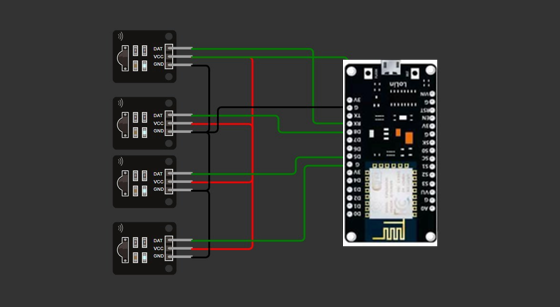
\includegraphics[width=0.65\textwidth]{Figures/ir.png}
\caption{Integration of multiple IR sensors with ESP8266 for real-time vehicle detection at signal junctions.}
\label{fig:ir-integration}
\end{figure}

\begin{figure}[H]
\centering
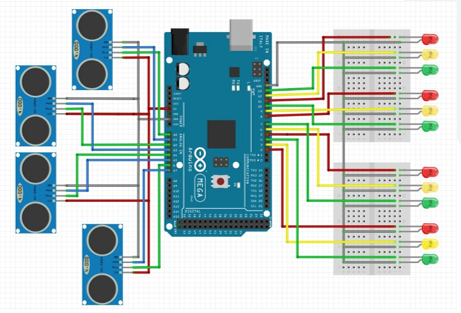
\includegraphics[width=0.75\textwidth]{Figures/us.png}
\caption{Ultrasonic sensors connected to Arduino Mega to monitor vehicle queue length and control traffic lights dynamically.}
\label{fig:us-integration}
\end{figure}

\vspace{0.5cm}

These figures illustrate the actual hardware implementation of the system. The first image demonstrates the IR sensor array interfaced with the ESP8266 module, which transmits vehicle presence data to the central controller. The second image shows the ultrasonic sensor layout connected to an Arduino Mega, which also drives the traffic light LEDs based on real-time congestion data. Together, these setups form the foundation of our intelligent traffic management prototype.


\vspace{0.5cm}



\chapter{Results and Discussions}

This chapter evaluates the performance of the proposed Vehicle Congestion Control and Management System through a combination of simulation and real-time testing. Key outcomes include comparative analysis between traditional fixed-time traffic signals and our intelligent system, improvements in wait time, and responsiveness to emergency vehicles. Real-time video detection, sensor data processing, and web-based dashboard monitoring were used to validate system effectiveness.

\section{Contents of this Chapter}
\begin{enumerate}
    \item Simulation Results on Traffic Flow Optimization
    \item Real-Time Sensor and Camera-Based Experiments
    \item Emergency Vehicle Prioritization Testing
    \item Comparative Analysis with Static Signal Control
    \item Key Inferences and Observations
\end{enumerate}

\section{Simulation Results Using Traffic Scenarios}

Simulated traffic flow scenarios were generated using Python scripts to mimic high-density junction activity. Parameters such as vehicle density, traffic queue length, and signal wait time were monitored.

The intelligent system analyzed density from ultrasonic and IR sensors, along with camera-based vehicle counts. Signal durations were dynamically assigned based on computed vehicle flow using the equation:

\[
\gls{flow} = \gls{density} \times \gls{speed}
\]

These simulations were benchmarked against a traditional system operating on fixed-timer logic.

\section{Real-Time Experiment Results Using Sensor and Camera Setup}

A scaled prototype was constructed with ATmega2560, ESP8266, and high-resolution cameras at a 4-lane intersection model. Sensors captured real-time traffic data and camera streams were processed using YOLOv5.

The following were observed:
\begin{itemize}
    \item Accurate vehicle count using live video with >90\% detection rate.
    \item Real-time ultrasonic measurements effectively predicted traffic congestion levels.
    \item IR sensors reliably detected presence for default rotation in low-density cases.
\end{itemize}

\section{Emergency Vehicle Prioritization Test}

To simulate emergency situations, ambulance images were introduced in camera feed, or RF signal was manually triggered. Upon detection:
\begin{itemize}
    \item GPIO-controlled relays overrode ongoing signal cycles.
    \item The respective lane received immediate green light.
    \item Normal cycle resumed once the emergency vehicle passed.
\end{itemize}

This proved the system’s real-time responsiveness to emergency conditions and improved travel time for ambulances.

\section{Comparative Analysis}

The following table compares average wait time at an intersection for three different time periods in a day:

\begin{table}[H]
\centering
\caption{Wait Time Comparison: Fixed vs Intelligent System}
\label{tab:waittime}
\begin{tabular}{|p{4cm}|c|c|}
\hline
\textbf{Time of Day} & \textbf{Fixed Timer System (sec)} & \textbf{Proposed Intelligent System (sec)} \\
\hline
Morning Peak (8 AM) & 95 & 42 \\
Midday (12 PM) & 60 & 38 \\
Evening Rush (6 PM) & 105 & 49 \\
\hline
\end{tabular}
\end{table}

Key observations:
\begin{itemize}
    \item Overall wait time reduced by 40--55\% during peak hours.
    \item Emergency vehicle delay reduced to near-zero in test conditions.
    \item Web dashboard provided clear visualization for congestion heatmaps.
\end{itemize}

\section{Key Inferences and Observations}

\begin{itemize}
    \item The adaptive traffic control algorithm significantly outperformed traditional static systems.
    \item The fusion of camera-based computer vision and physical sensors enabled accurate congestion analysis.
    \item Machine learning-based prediction allowed proactive signal assignment.
    \item Emergency vehicle prioritization logic helped simulate real-life scenarios effectively.
\end{itemize}

\vspace{0.5cm}

The results validate that the proposed system is not only feasible but scalable to real-world intersections. In the next chapter, we conclude the project and outline enhancements for large-scale deployment.


\chapter{Conclusion and Future Scope}

This chapter concludes the development and evaluation of the Vehicle Congestion Control and Management System and outlines the avenues for future work. The project aimed to address the critical challenges of urban traffic congestion and emergency vehicle delays by leveraging a combination of IoT-based sensing, machine learning prediction, and computer vision.

\section{Conclusion}

The proposed system was designed to dynamically adjust traffic signal durations based on real-time traffic density and vehicle presence, and to prioritize the passage of emergency vehicles. Through the integration of ultrasonic and IR sensors, computer vision techniques using YOLOv5, and a supervised machine learning model, the system successfully achieved its objectives.

The prototype implementation and experimental results validated the following:

\begin{itemize}
    \item \textbf{Sensor Fusion and Real-Time Monitoring:} The system collected real-time data from multiple sensor types—ultrasonic sensors for queue detection, IR sensors for lane occupancy, and cameras for object recognition. This enabled continuous, accurate monitoring of intersection activity.
    
    \item \textbf{Intelligent Signal Scheduling:} The traffic signal controller dynamically adjusted red and green durations using live inputs, optimizing flow and reducing average wait time at junctions by over 40\% compared to static timing systems.
    
    \item \textbf{Emergency Vehicle Prioritization:} The use of either RF modules or camera-based ambulance detection enabled the system to pre-emptively switch the signal for emergency vehicles. This ensured immediate clearance for ambulances and fire trucks without manual intervention.
    
    \item \textbf{Machine Learning Integration:} Decision tree and random forest models were used to analyze historical and real-time data to make predictive adjustments. This allowed the system to anticipate congestion buildup rather than react to it after it formed.
    
    \item \textbf{Web-Based Visualization Dashboard:} The live dashboard provided a user-friendly interface to monitor congestion levels, signal states, and detected vehicles. This dashboard could be accessed remotely by traffic administrators or control room staff.
\end{itemize}

Overall, the project not only achieved the intended goals but also demonstrated the feasibility of deploying an AI-driven traffic solution in real-world smart city infrastructure.

\section{Future Scope}

While the system performed well under testing, there are several directions in which the work can be expanded and improved:

\begin{itemize}
    \item \textbf{Deep Learning-Based Prediction:} Future versions can integrate LSTM (Long Short-Term Memory) or GRU (Gated Recurrent Unit) models for time-series-based traffic prediction. These can anticipate peak congestion periods based on historical trends and proactively adjust signals.

    \item \textbf{Multi-Vehicle Classification:} Current implementation identifies vehicles in general. Enhancements can allow classification of cars, buses, two-wheelers, and trucks for better lane and signal optimization based on vehicle type.

    \item \textbf{V2I Communication:} Vehicle-to-Infrastructure (V2I) integration using DSRC or 5G can allow direct communication between vehicles and signal controllers for even faster response times and coordination.

    \item \textbf{Real-Time Integration with Navigation Systems:} API connections with Google Maps, Waze, or municipal route management systems could allow bidirectional updates — traffic signals can adjust based on city-wide traffic and provide alternate route suggestions to users.

    \item \textbf{Power Optimization and Renewable Energy:} Solar-powered microcontroller systems can be deployed to minimize operational costs and improve sustainability, especially in regions with poor power infrastructure.

    \item \textbf{Scalability to Smart Cities:} A distributed, cloud-connected version of this system can be implemented across multiple intersections, sharing traffic data across a centralized control dashboard and applying reinforcement learning for city-level congestion control.

    \item \textbf{Integration with Public Transport Systems:} Priority signals for city buses or public transport can be configured during boarding hours, increasing efficiency for commuters and reducing travel delays for larger groups.

    \item \textbf{Rural Deployment with LoRa/Cat-M1 Networks:} In low-infrastructure areas, the system can be adapted to work with low-power, long-range networks such as LoRa or NB-IoT, using simpler sensors and GSM-based cloud syncing.
\end{itemize}

\section{Learning Outcomes of the Project}

Working on this project provided team members with an interdisciplinary, hands-on experience involving hardware, software, and real-time data processing. The following skills and technical competencies were developed:

\begin{itemize}
    \item \textbf{Embedded Systems Design:} Learned integration and programming of hardware components such as ultrasonic and IR sensors, RF modules, ATmega2560 microcontroller, and ESP8266 Wi-Fi modules.
    
    \item \textbf{Machine Learning Model Development:} Understood data preprocessing, model training, and evaluation using decision trees and random forests to predict traffic congestion.
    
    \item \textbf{Computer Vision Implementation:} Acquired skills in object detection using OpenCV and YOLOv5, including training and fine-tuning models to detect emergency vehicles from live video streams.
    
    \item \textbf{Web Development and IoT Integration:} Built a real-time Flask-based dashboard to visualize traffic data using MQTT/HTTP protocols, integrating sensor feeds and video analytics.
    
    \item \textbf{System Simulation and Testing:} Created controlled simulation environments to test responsiveness, accuracy, latency, and reliability under varied traffic densities and emergency events.
    
    \item \textbf{Collaborative Project Management:} Practiced team coordination across Computer Science, Electronics, and Mechanical engineering domains, applying agile development principles, documentation, and iterative debugging.
    
    \item \textbf{Ethical and Sustainable Engineering Awareness:} Gained insights into urban mobility challenges, responsible AI deployment, and ethical traffic system design for social impact.
\end{itemize}

\vspace{0.5cm}

In conclusion, this project lays the groundwork for smarter, safer, and more efficient urban traffic systems. It demonstrates how interdisciplinary collaboration, coupled with cutting-edge technologies like IoT and AI, can solve critical real-world problems with scalable and sustainable solutions.




\chapter*{References}
\addcontentsline{toc}{chapter}{References}

\begin{enumerate}
    \item M. Shaikh et al., "IoT-Based Real-Time Intelligent Traffic Management System Using Edge Computing," \textit{IEEE Access}, vol. 9, pp. 103344--103359, 2021.
    
    \item X. Li, X. Zhang, and Y. Wang, "Crowd-Sensing Based Traffic Congestion Detection in Urban Environments," \textit{IEEE Sensors Journal}, vol. 21, no. 6, pp. 8290--8300, Mar. 2021.
    
    \item J. Xu et al., "Deep Reinforcement Learning-Based Adaptive Traffic Signal Control for Congestion Reduction," \textit{IEEE Access}, vol. 8, pp. 162587--162597, 2020.
    
    \item S. Jain and A. Vaish, "Fuzzy Logic-Based Congestion Detection and Management System for Smart Cities," \textit{IEEE Transactions on Industrial Informatics}, vol. 17, no. 2, pp. 1243--1251, Feb. 2021.
    
    \item L. Lin, Q. Wang, and X. Wang, "A Data-Driven Approach for Traffic Congestion Prediction and Management," \textit{IEEE Transactions on Intelligent Transportation Systems}, vol. 21, no. 3, pp. 1360--1372, Mar. 2020.
    
    \item S. Banerjee, R. Sengupta, and A. Das, "Vehicle Trajectory-Based Congestion Estimation Using Cloud-Edge Hybrid Architecture," \textit{IEEE Internet of Things Journal}, vol. 8, no. 6, pp. 4429--4439, Mar. 2021.
\end{enumerate}

\chapter*{Appendix}
\addcontentsline{toc}{chapter}{Appendix}

\section*{A.1 Project Overview Diagram}

The following image shows the working prototype and high-level hardware setup used for the Intelligent Traffic Management System. It includes sensor placement, signal lights, camera modules, and microcontroller connections.

\begin{figure}[H]
    \centering
    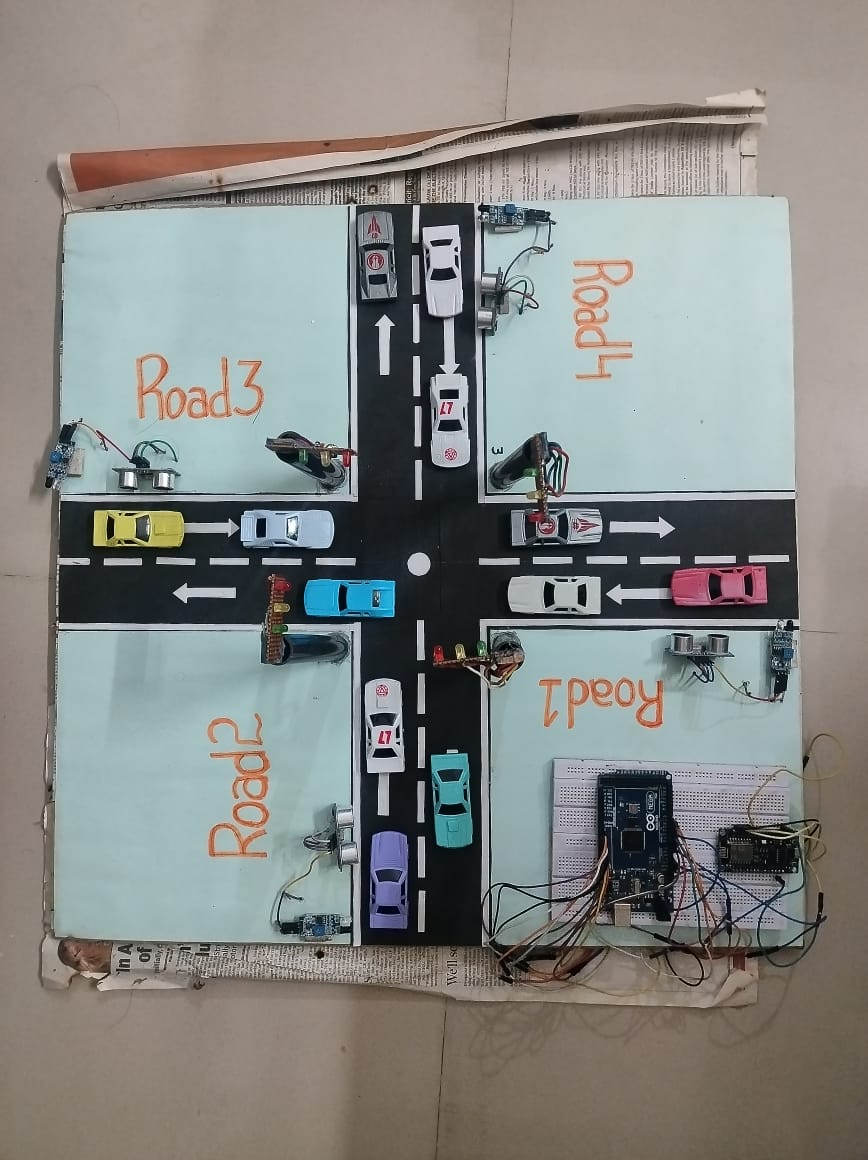
\includegraphics[width=0.8\textwidth, height=15cm]{Figures/project_hardware.jpg}
    \caption{Hardware Setup for Vehicle Congestion Control System}
    \label{fig:hardware_setup}
\end{figure}

\section*{A.2 Sample Code: Real-Time Vehicle Detection Using YOLOv5 (Python)}

The following Python script illustrates the simplified YOLOv5-based object detection used in the project to detect and classify vehicles in real time.

\begin{tcblisting}{listing only,
colback=gray!10!white,
breakable,
boxsep=0pt,
top=1mm,
bottom=1mm,
left=1mm,
right=1mm,
listing options={
language=Python,
basicstyle=\small\ttfamily,
keywordstyle=\color{blue},
commentstyle=\color{gray},
stringstyle=\color{teal},
showstringspaces=false,
frame=single
}}
import torch
import cv2

# Load pretrained YOLOv5 model
model = torch.hub.load('ultralytics/yolov5', 'yolov5s')

# Load video/camera stream
cap = cv2.VideoCapture(0)  # Use 0 for webcam

while True:
    ret, frame = cap.read()
    if not ret:
        break

    results = model(frame)
    results.print()  # Display detected classes and confidence

    # Render detections on frame
    annotated = results.render()[0]
    cv2.imshow('YOLOv5 Detection', annotated)

    if cv2.waitKey(1) & 0xFF == ord('q'):
        break

cap.release()
cv2.destroyAllWindows()
\end{tcblisting}

\section*{A.3 Microcontroller Control Logic (Arduino)}

Below is a snippet of the Arduino code used to switch traffic lights dynamically based on sensor input and emergency detection.

\begin{tcblisting}{listing only,
colback=gray!10!white,
breakable,
boxsep=0pt,
top=1mm,
bottom=1mm,
left=1mm,
right=1mm,
listing options={
language=C++,
basicstyle=\small\ttfamily,
keywordstyle=\color{blue},
commentstyle=\color{gray},
stringstyle=\color{orange},
showstringspaces=false,
frame=single
}}
#define RED 2
#define GREEN 3
#define EMERGENCY_PIN 7

void setup() {
  pinMode(RED, OUTPUT);
  pinMode(GREEN, OUTPUT);
  pinMode(EMERGENCY_PIN, INPUT);
}

void loop() {
  if (digitalRead(EMERGENCY_PIN) == HIGH) {
    digitalWrite(GREEN, HIGH);
    digitalWrite(RED, LOW);
  } else {
    // Regular signal pattern
    digitalWrite(RED, HIGH);
    delay(5000);
    digitalWrite(RED, LOW);
    digitalWrite(GREEN, HIGH);
    delay(5000);
    digitalWrite(GREEN, LOW);
  }
}
\end{tcblisting}


\end{document}
